%!TEX root = ../master_thesis.tex

\chapter{Case study}
\label{chapter:case_study}

In this chapter we describe the case study and explain how the terminology model we proposed in previous \nref{sec:software_environment_terminology} relates to it. We re-state our problem in the context of the case study, highlight the evolution of architecture in the case study and introduce the concrete implementations of infrastructure systems, which are relevant to our work in later chapters.

In the first quarter of 2014, the author worked with SoundCloud~\cite{soundcloud} in the context of this work. SoundCloud produces one product, which they describe as ``the world’s leading social sound platform where anyone can create sounds and share them everywhere''~\cite{soundcloudabout}. In October 2013 it had 250 million monthly active listeners \cite{soundcloudusers}. On May 9th 2014, the Alexa Global Rank of the product was 166 \cite{alexasoundcloud}. In April 2013, the company had 190 employees in four offices (Berlin, London, San Francisco, Sofia) with 80 engineers mainly located in the Berlin office~\cite{soundcloudAG}.

In the deployed microservice architecture of the case study we found hundreds of applications and thousand of processes deployed in the productive environment.
One of the problems that became apparent to us while interviewing engineers as well as through observing the day-to-day work in the company was that there did not exist a holistic understanding of how applications and processes relate to each other. Often not even the immediate dependencies of applications were clear to engineers, manifesting themselves in the two questions ``Which applications does my application depend on?'' and ``Which applications depend on my application?''. Resulting from these observations, we especially found the question of how failures propagate through the system to be an interesting angle for research.

Before we discuss our solutions to these problems in the following chapters, we will discuss the technical environment of the case study more closely.

% A note of caution: The nature of development in our case study was optimized for high velocity, which means that systems might change rapidly. Therefore the information we present here is a snapshot and is likely to have changed already again by the release of this works.

\section{Architectural style}
\label{sec:architecture}

We separate the product into two big categories: \emph{clients} and the \emph{platform}. The clients are software that is executed within the realm of the human users. This software may be the website on \emph{soundcloud.com} running in a web browser, native applications (mostly on mobile devices) or consumers of the public REST API~\cite{soundclouddevelopers}~\cite{Fielding}. The client software may be developed by the company or by third parties. All clients interact with the platform via APIs based on the HTTP protocol~\cite{rfc2616}. Usually the clients functionality is tightly bound to the functionality provided by the platform. In fact they might provide no functionality at all if there is no connectivity to the platform. Clients are not the focus of this work and will not be represented in further investigations. This is based on the notion that due to the context of the execution of clients we do not see them as part of the microservice architecture, even though they technically consume services provided by the microservice architecture. Figure \ref{fig:evolution_example} shows how clients and platform relate to each other.

The \emph{platform} is implemented as a \emph{multi-user} \emph{Software as a Service}. Thus, the software, the runtime resources and the user data are managed by the company. The platform is implemented as \emph{multi-user}, meaning that all users use the same computing and data storage resources.

The development of the platform started in 2007. Since then, it has been incrementally developed further in evolutionary steps, which we will describe next:
\begin{tdescription}
  \item[1. Monolithic application] Initially, the platform development started with the \emph{Ruby on Rails}~\cite{Rails} web development framework. All presentation and business logic was concentrated in one monolithic application, which was executed with one process type and many process instances. One database system held all data.
  \item[2. Splitting the monolithic application] Starting 2010, functionality started to be moved out of the monolithic application and into independent applications \cite{Phil2013Monolith} \cite{EvolutionTreadway}. These applications might still have major functional dependencies on the business logic of the monolithic application. New features are not developed in the monolithic application anymore, but as new applications. We see the case study being currently in this stage, since the monolith still carries major significance.
  \item[3. Full microservice architecture] The goal of the architecture evolution is to reduce the significance of the monolith to ``just being another service''. Thus, the functionalities of the platform as a whole should be split relatively equally over all applications. A platform that is developed further towards this style is Twitter, introduced in \cite{twittersoa}.
\end{tdescription}

Figure \ref{fig:evolution_example} visualizes these three evolution steps.

\begin{figure}[h!]
  \centering
  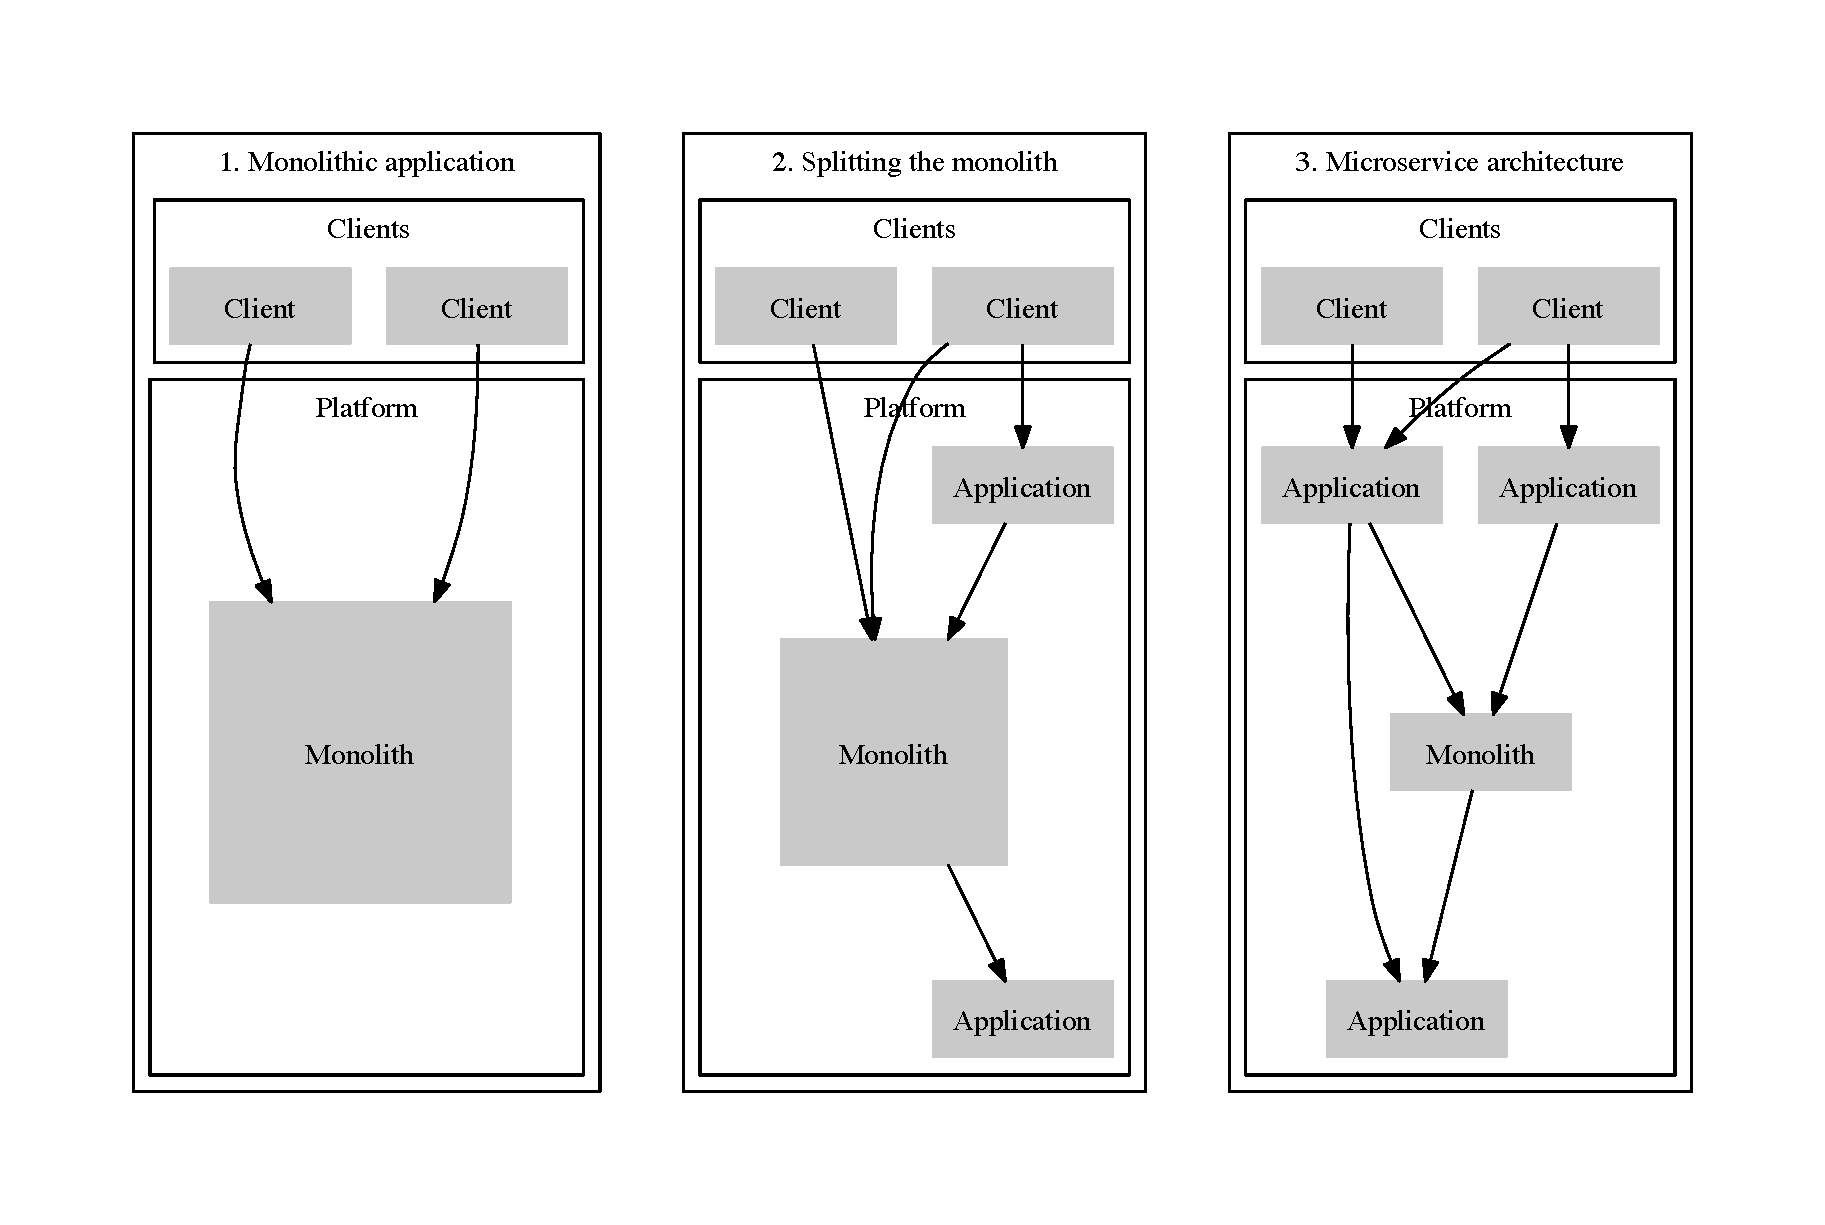
\includegraphics[width=\linewidth] {images/arch-evolution.pdf}
  \caption{Visualization of the architecture style evolution from monolithic architecture style to microservice architecture style. Boxes represent applications and directed edges represent service dependencies. Size of the ``monolith'' represents its significance in the architecture.}
  \label{fig:evolution_example}
\end{figure}

We see two major drivers for this evolution:
\begin{tdescription}
  \item["The right tool for the job"] Different functionalities require different approaches to implement them efficiently. These approaches may be hard to consolidate in one application, most notably since different programming languages or frameworks might be used.
  \item[De-coupling of development and deployment] Small teams of 2 - 10 people are believed to work more effectively than bigger teams \cite{HenrikKniberg}. Conway's law~\cite{conway} suggests that the structure of a system designed by an organization will follow the organization's communication structure. Following this law, it is logical to assume that as an engineering organization grows with many small teams, the architecture will follow the same style. As a side benefit, small teams and applications allow for easier and therefore more often application deployment, which in turn increases the velocity and quality of software \cite{fowler-microservices} \cite{ContinuousDelivery}.
\end{tdescription}

During our investigations we noted that the development of the architecture was not centrally controlled but rather happened to the discretion of individual engineers. Every engineer was able to decide how functionalities should be split into different applications. This led to a lack of oversight over the architecture development in the engineering organization. During our investigations we also found many different technologies in use for developing applications. For example we found 9 different programming languages used in the case study (as further explained in \nref{subsec:from_smi}, especially Table \ref{tab:SIM_language_stats}).

\subsection{Technical details}
\label{subsec:case_study_tech_details}

In this section we cover some technical details of the case study.

All codebases were organized with the Git~\cite{ProGit} source code versioning system. The canonical location for all repositories is at GitHub~\cite{github}, which is a SaaS providing Git repository hosting.
In our case study, all repositories were organized within one ``GitHub organization''~\cite{ghorgs}, which is a logical grouping of hosted repositories, providing centralized access control and billing. We provide more statistics over repositories and their usage in later  \nref{subsec:graph_manual_annotation}.

All repositories on Github have an identifier. Since each application has a canonical Github repository and since these are unique, we may use the repository identifiers as application identifiers as well. We found two cases where a repository contained several applications. In these cases we assigned that repository to several applications with different identifiers\footnote{One of the cases is described later in \autoref{sec:case_study_execution}}.

% \subsubsection{Inter-process communication}
%
% In our case study, all inter-process communication happens
%
% Network communication is the way for inter-process communication in the case study. The internet protocol suite (most notably TCP/IP~\cite{internetprotocol}) was the common basis for network communication. As application layer protocol HTTP~\cite{rfc2616} was the most commonly used.

In our case study, machines were distributed over several company-operated datacenters as well as rented cloud platforms. Several different Linux distributions were in use.

\section{Infrastructure systems}

Next we will describe the systems for \emph{deployment}, \emph{service discovery} and \emph{telemetry} that we found in our case study.

\subsection{Deployment systems}
\label{subsec:deploymentsys}

In our case study we found various systems facilitating deployments. We introduce \emph{Bazooka}, which is a ``Platform as a Service'' (short: PaaS) for deploying stateless applications, and \emph{Chef}, which is a machine configuration system that is used for deploying stateful applications.

\subsubsection{Bazooka}

Bazooka~\cite{bazookaTalkGoto} is a ``Platform as a Service'' deployment system. It is similar to the hosted PaaS Heroku~\cite{heroku} and Google App Engine\cite{GAE}, as well as the self-hosted PaaS Mesos~\cite{mesos}, Flynn~\cite{flynn} and Deis~\cite{Deis}. Among others Bazooka handles the building of deployment artifacts, resource allocation for job scheduling, process supervision, service discovery setup, request handling and load balancing, as well as monitoring and logging.

Bazooka facilitates the deployment of applications on internal resources. It was built for applications that expose services via HTTP. The applications need to adhere to the constraints of ``12 factor''~\cite{12factor}. ``12 factor'' is based on observations made by Wiggins regarding the design of applications in the context of the PaaS Heroku~\cite{heroku}. The developers of Bazooka adopted these constraint for their platform as well. The constraints relevant in the context of our work are as following:
\begin{titemize}
  \item All applications' codebases are tracked in Git~\cite{ProGit}.
  \item All processes are ``stateless'', meaning that they hold no persistent data. This alleviates the need for a data consistency model between processes. Also, data locality and durability are no concerns. This constraint allows for near-linear horizontal scaling, meaning that double the amount of service instances should allow for handling double the amount of requests per second.
\end{titemize}

Bazooka consists of the following components:
\begin{tdescription}
  \item[Bazooka repository manager] handles the building of the applications.
  \item[Bazooka application host] provides the computing resources to run the processes and manages the life cycle of the processes.
  \item[Bazooka proxy] manages service discovery and request routing to processes.
\end{tdescription}

If an engineer wants to deploy an application with Bazooka, they first have to go through an initial setup. They create a Bazooka application on the Bazooka repository manager. The identifier of the Bazooka application is the same as the repository name and has to be unique. Next, a Bazooka configuration for the application is created. Each configuration is a set of key-value pairs, which at runtime are available to the application via operating system environment variables. The current state of the Bazooka system, including applications, configurations and running processes, is managed via Doozer~\cite{Doozer}, a distributed, consistent data store.

The process of deploying an application with Bazooka is as follows: The engineer pushes the codebase to a git remote\footnote{A git remote is a git repository that is hosted somewhere else than the current repository. It is possible to push and pull changes from git remotes, in order to share file changes. For more information, see \cite{ProGit} Section 2.5.} on the Bazooka repository manager. There a deployment artifact is built (usually described via a Makefile~\cite{make})\footnote{It is also possible to deploy already-built artifacts.}. Once the building procedure is completed the engineer may start processes from the deployment artifact. Each deployment artifact is referenced with a revision\footnote{This is either the git commit identifier hash string or a revision string assigned by the Bazooka repository manager for the deployment artifact.}. When a process instance is started, the deployment artifact for it is transferred to the appropriate Bazooka application hosts, the process instance is started in the operating system and the running service is included in the service discovery.

At the time of writing, Bazooka was the preferred way of deploying microservices in our case study. On March 14th 2014, the deployment of Bazooka in our case study had 1 Bazooka repository manager, 2 Bazooka load balancers and 45 Bazooka application hosts, with 211 application deploys running 1333 processes~\footnote{This includes staging and testing deploys as well as prototypes and infrastructure applications}.

% Future goal: job scheduling for using resources efficiently. Processes have different usage profiles (high memory, low CPU), so trying to locate processes in a way that resources are well-used.

\subsubsection{Chef}

\emph{Chef} describes itself as ``a systems and cloud infrastructure automation framework that makes it easy to deploy servers and applications to any physical, virtual, or cloud location [...]''~\cite{chefdocs} as well as ``a configuration management tool designed to bring automation to your entire infrastructure.''~\cite{chefgithub}. A configuration is the state of an architecture at a point in time. The configuration that Chef uses is described in code. This might include setting up a file structure, installing and managing applications or collecting and rendering configuration files.

\emph{Chef} has a central Chef server that manages the configuration code, and a Chef client process on each managed machine. The highest granularity in Chef to manage machines is ``roles''. A machine might have many roles assigned. Each role has code associated which gets executed in order to configure the machine. The Chef server allows to query which roles are applied to which machines. Conversely it is possible to fetch the applied roles from each machine via its Chef client.

In our case study, Chef is used to deploy all infrastructure applications. For example the components of the \emph{Bazooka} deployment system get deployed themselves via Chef. \emph{Chef} is also used for deploying applications which are stateful and therefore can not be deployed via \emph{Bazooka}.

% Stateful: holds state. usually both in a non-permanent storage (memory) and permanent (disk). State has to be kept consistent, therefore scaling out becomes more difficult. Also data management (storage, backup) has to happen.

% \subsubsection{Other}
%
% Capistrano. Preparation of the sever via chef beforehand.
% Capistrano. Deployment from the perspective of the application.
% Deployment of main monolithic application

\subsection{Service Discovery}
\label{subsec:servicediscovery}

Service discovery is the procedure of finding the process instance locations for a specific deploy. In our case study we found four service discovery mechanisms: \emph{physical addresses}, \emph{semantic DNS CNAMEs}, \emph{Bazooka} and \emph{Glimpse}. When describing service discovery mechanisms, one is often interested in attributes like propagation delays, load balancing or fault tolerance \cite{servicediscoverysurvey}. In our investigations, we are only interested in how the mappings between service discovery key and locations work. We will make extensive use of mechanisms introduced here in later \nref{chapter:dependency_graph}.

\subsubsection{Physical Addresses}

Under physical address we understand two methods:
\begin{tenumerate}
  \item the \textbf{IP address} directly like \lstinline{10.20.103.02}; or
  \item a \textbf{physical domain name} denoting the machine directly without application semantics like \lstinline{app08.internal.example.com}.
\end{tenumerate}

In both cases, the port numbers of the services for each address have to be known as well, in order to make a connection to a service. Physical domain names are registered and resolved via the DNS Domain Name System \cite{rfc1591}.

IP address and physical domain name are usually assigned when a machine is initially integrated into the company environment. We expect these assignments to not change\footnote{Physical machines may get re-assigned. In our terminology this would constitute the decommissioning of the old machine and integration of a new machine. Also \emph{Virtual IP addresses} were in use in the case study to provide fault tolerance capability on the traffic layer as well as for load balancing reasons. These were exceptions and we did not include them in our investigations.}.

Both methods may be seen as not constituting real service discovery. Even though for the physical domain name there is one DNS resolution step, it has no semantic meaning and therefore in our investigations does not add service discovery value.

We found both methods to be commonly used in our case study. The also are the final resolution step for the other methods, since they allow the actual addressing of machines and services via the network.

\subsubsection{Semantic DNS CNAME}

Apart from the physical domain names, we also found semantic domain names in use, defined via DNS CNAME records following the pattern of \lstinline!{name}.internal.example.com!. These are configured manually by engineers, and map to one IP address. As with physical domain names, these do not include port numbers, which have to be known already.

Even though the usage of this method is discouraged, it is still in use (as we will show in later \nref{subsec:graphfromdeploymentconf}). We attribute its use to the simplicity of registering and querying the domains.

\subsubsection{Bazooka}
\label{subsubsec:service_disco_bazooka}

The preferred way of reaching services deployed with Bazooka is via the Bazooka load balancers. When an application is initially registered with Bazooka, each of its services gets assigned a port number. The services keep their port numbers indefinitely, therefore these are the service discovery contracts with the consumers. A consumer may use the service by requesting a Bazooka load balancer on the application's port number. The load balancer will then forward the request to one of the service instances.

Bazooka has several load balancer instances (at the time of writing it were 2 with plans to use more in the near future). All instances share the same configuration mapping between port numbers and the service instances available for each of these port numbers.

The Bazooka load balancers may be addressed via one of the other service discovery methods. The most common method we found during our investigations (as explained later in \nref{subsec:graphfromdeploymentconf} and \nref{subsec:from_network}) was via semantic CNAMEs. Figure \ref{fig:bazooka_lb_sd_example} shows an example of addressing a service instance with the request flow from the service consumer to a service instance.

\begin{figure}[h!]
  \centering
  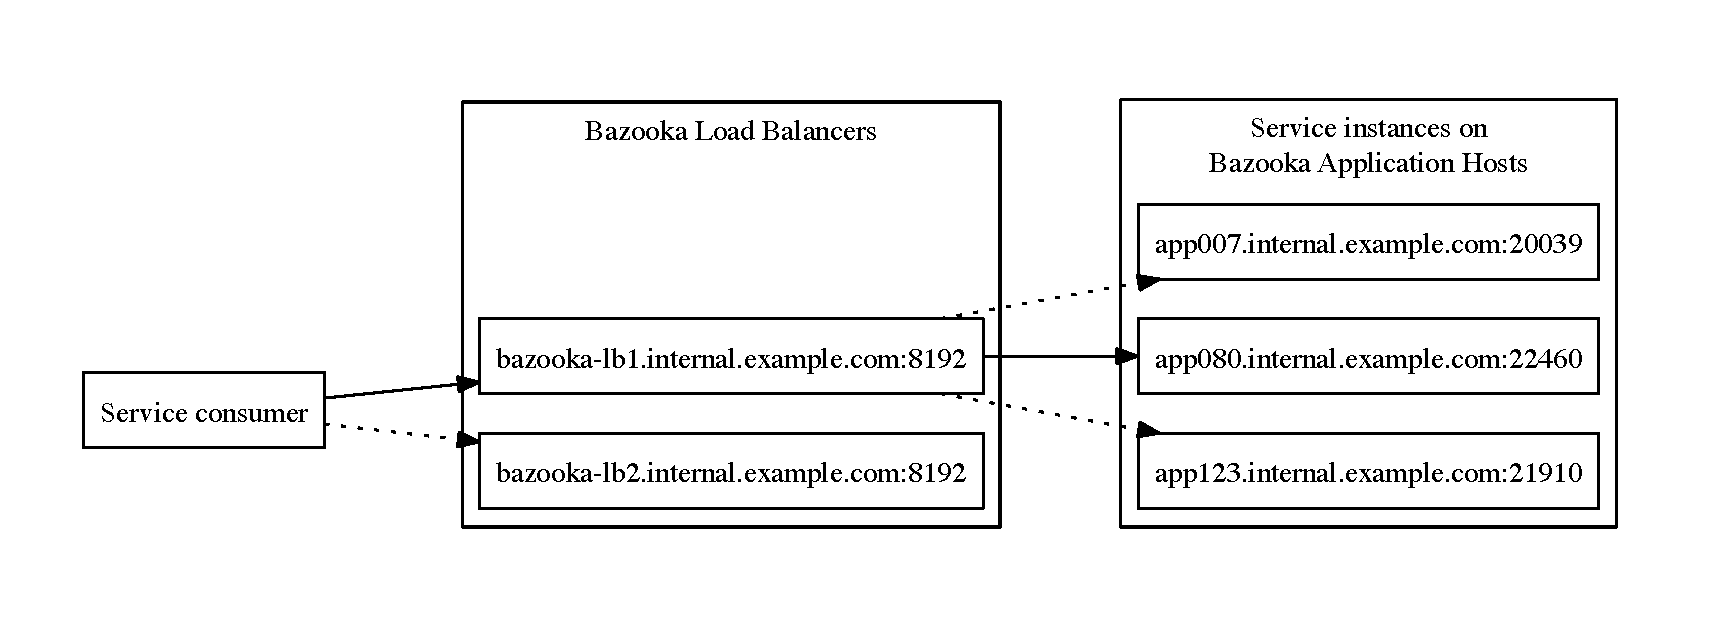
\includegraphics[width=\linewidth] {images/bazooka-lb-service-discovery.pdf}
  \caption{Visualization of the request flow from client to service through the Bazooka load balancer. Boxes represent machines with the domain name and port number as names. Solid edges represent the request flow. Dotted edges represent potential opportunities for different request flows, which would still yield the same results.}
  \label{fig:bazooka_lb_sd_example}
\end{figure}

\subsubsection{Glimpse}
\label{subsubsec:glimpse}

Glimpse is an application for service discovery, developed in-house of our case study. It is based on DNS SRV records (specified in RFC 6763~\cite{rfc6763}), which for one domain name allow to request many pairs of domain name and port number. The query domains have the following format:

\lstinline!{protocol}.{job}.{env}.{product}.{zone}.internal.example.com!
\begin{tdescription}
  \item[protocol] denotes the application-layer protocol with which to access the service. Examples are \emph{http} or \emph{ssh}.
  \item[job] is the name of the service in the context of the application. Examples are \emph{web} or \emph{admin}.
  \item[env] is the environment of the application deploy. Examples are \emph{production} or \emph{staging}.
  \item[product] denotes a grouping of user stories. It might match an application and repository name, but there is no convention enforcing that.
  \item[zone] denotes the zone, which a logical grouping of computing resources. Zones might for example be used to differentiate data centers.
\end{tdescription}

An example domain name is \\ \lstinline{http.app.prod.soundcloud.ca.srv.internal.example.com}

An example query is shown in \autoref{list:glimpsequeryexample}.

\begin{lstlisting}[caption=Service discovery via Glimpse; Query example ,label=list:glimpsequeryexample,numbers=none]
$ dig +short SRV http.app.prod.soundcloud.ca.srv.internal.example.com
0 0 5023 app117.internal.example.com
0 0 5023 app118.internal.example.com
0 0 5024 app097.internal.example.com
0 0 5024 app117.internal.example.com
\end{lstlisting}

The service discovery requests of Glimpse are handled via BIND~\cite{bind} DNS server. At the time of writing, two existed, which are the authoritative sources for the Glimpse DNS namespace. The namespaces are initially configured by engineers, but the actual service instance information for each glimpse domain is gathered and distributed to the DNS server automatically.

% Might also be used for bazooka deployed

% To summarize this section, table XXX shows for each method the mapping between one application name, respective intermediate formats and the eventual ipaddress:portname combinations.
%
% \begin{table}
%   \caption{Examples for the explained service discovery methods}
%   \label{tab:shortened_app_names}
%   \begin{tabular}{ |l|l|l| }
%     \hline
%     Service discovery key & Intermediate representation & Service location(s) \\
%     \hline
%     Physical Address (IP) \\
%     10.20.30.40 & & 10.20.30.40:2000 \\
%     \hline
%     Physical Addresses (Name) \\
%     app08.internal.example.com & 10.20.30.40 & 10.20.30.40:2000 \\
%     \hline
%     Semantic DNS CNAME \\
%     app.internal.example.com & app08.internal.example.com & 10.20.30.40:2000 \\
%     \hline
%     Bazooka \\
%     bazooka-lb.internal.example.com:3001 & 10.20.30.40:3001 (Bazooka load balancer) & 10.20.30.40:2000 \newline 10.20.30.41:2000 \\
%     \hline
%     Glimpse \\
%     http.web.prod.app.ca.srv.internal.example.com & & \\
%     \hline
%   \end{tabular}
% \end{table}

\subsection{Telemetry}
\label{subsec:telemetry}

Telemetry systems measure the state of a system, collect this information and make it available to engineers. During our investigations they were crucial tools for understanding and reasoning about the deployed architecture. Here we present three telemetry systems that were in use in our case study. More systems do exist, but we limit our descriptions to the ones that were relevant to our investigations.

\begin{tdescription}
  \item[Graphite]\cite{graphite} describes itself as doing two things: ``1. Store numeric time-series data 2. Render graphs of this data on demand''. Every time series consists of many datapoints. A series has a resolution, defining how many seconds of time each datapoint covers. In our case study, the standard resolution was 60 seconds. Data is sent to \emph{Graphite} via HTTP, setting the value for individual data points in time series. During querying, time series may be transformed and combined through functions. Graphite allows the extraction of the raw time series data as well as displaying visual graphs. In our case study, the majority of measures were collected and displayed with Graphite.
  \item[StatsD]\cite{statsd} describes itself as ``[a] network daemon that [...] listens for statistics, like counters and timers, [...] and sends aggregates to [...] backend services (e.g. Graphite)''. \emph{Graphite} only allows setting absolute numeric values for each datapoint. \emph{StatsD} allows for aggregating data for each datapoint before, for example when an event (like an HTTP request) happens, its result might be sent to \emph{StatsD}, which aggregates all of these events for the current datapoint and then sends that aggregated datapoint to \emph{Graphite}.
  \item[Prometheus]\cite{prometheus} describes itself as ``a generic time series collection and computation server''. Different to \emph{Graphite}, its data collection mechanism is pull-based: in regular intervals the \emph{Prometheus} server queries a telemetry HTTP resource on each measured instance. The instances internally aggregate the metrics.
\end{tdescription}

In our case study, \emph{Prometheus} is set to eventually replace the combination of \emph{Graphite} and \emph{StatsD}. At the time of our investigation, both systems were in use and served different measurements.

\section{Summary}

In this chapter we have introduced our case study, the berlin-based company ``SoundCloud'' in which the author was embedded while investigating this work. We have shown how the architectural style used in the case study has evolved from a monolithic multi-tier web application towards a microservice architecture (as visible in \autoref{fig:evolution_example}). We have also described concrete implementations of infrastructure systems, on which we will rely in the following chapters. As a problem in assessing the dependability of the deployed microservice architecture we identified a lack of visibility regarding the dependencies between applications.
